\documentclass{standalone}

\begin{document}

    \section{Sparkling Water Introduction}

    Sparkling Water allows users to combine the fast, scalable machine learning algorithms of H2O with the capabilities
    of Spark. With Sparkling Water, users can drive computation from Scala, R, or Python and use the H2O Flow UI, providing
    an ideal machine learning platform for application developers.

    Spark is an elegant and powerful general-purpose, open-source, in-memory platform with tremendous momentum. H2O
    is an in-memory application for machine learning that is reshaping how people apply math and predictive analytics to
    their business problems.

    Integrating these two open-source environments provides a seamless experience for users who want to pre-process data
    using Spark, feed the results into H2O to build a model, and make predictions. Sparkling Water tries to follow Spark
    conventions for the H2O algorithms so the API is easy to start with for people familiar with Spark.

    For end-to-end examples, please visit the Sparkling Water GitHub repository at {\url{https://github.com/h2oai/sparkling-water/tree/master/examples}}.

    \begin{minipage}{\textwidth}
        \textbf{Have Questions about Sparkling Water?}
        \setlength{\parskip}{1em}
        \begin{itemize}
            \setlength\itemsep{1pt}
            \item Post them on Stack Overflow using the \textbf{sparkling-water} tag at {\url{http://stackoverflow.com/questions/tagged/sparkling-water}}.
            \item Join the chat at {\url{https://gitter.im/h2oai/sparkling-water}}.
        \end{itemize}
    \end{minipage}

    \subsection{Typical Use Cases}
    Sparkling Water excels in leveraging existing Spark-based workflows needed to call advanced machine learning
    algorithms. We identified three of the most common use-cases which are described below.

    \subsubsection{Model Building}
    A typical example involves multiple data transformations with the help of Spark API, where a final form of data is
    transformed into an H2O frame and passed to an H2O algorithm. The constructed model estimates different metrics based
    on the testing data or gives a prediction that can be used in the rest of the data pipeline (see Figure~\ref{fig:use-case-1}).
    \begin{figure}[h!]
        \centering
        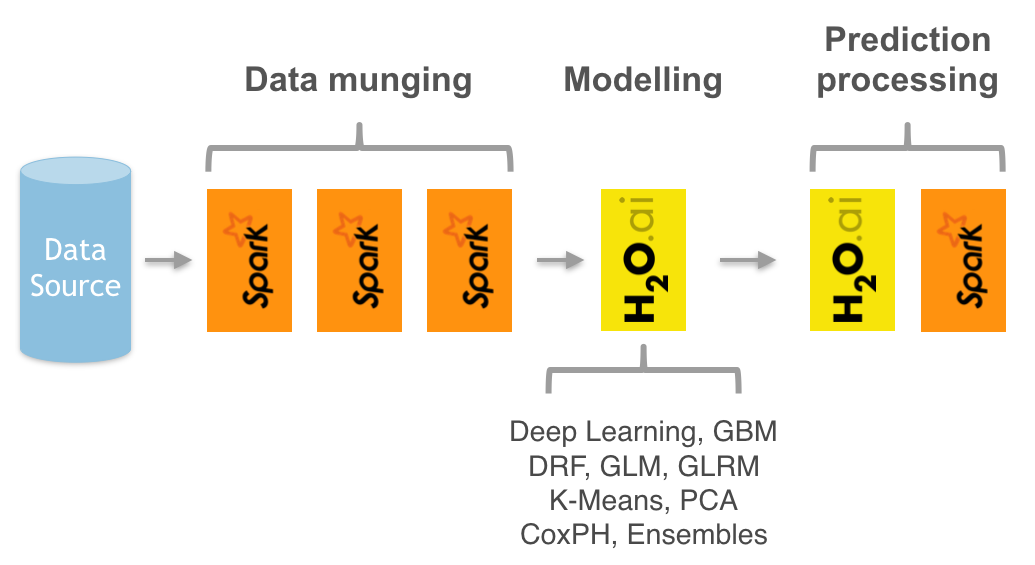
\includegraphics[scale=0.3]{../images/use-case-1.png}
        \caption{Sparkling Water extends existing Spark data pipeline with advanced machine learning algorithms.}
        \label{fig:use-case-1}
    \end{figure}

    \subsubsection{Data Munging}
    Another use-case includes Sparkling Water as a provider of ad-hoc data transformations. Figure~\ref{fig:use-case-2} shows
    a data pipeline benefiting from H2O's parallel data load and parse capabilities, while Spark API is used as another
    provider of data transformations. Furthermore, H2O can be used as an in-place data transformer.

    \begin{figure}[h!]
        \centering
        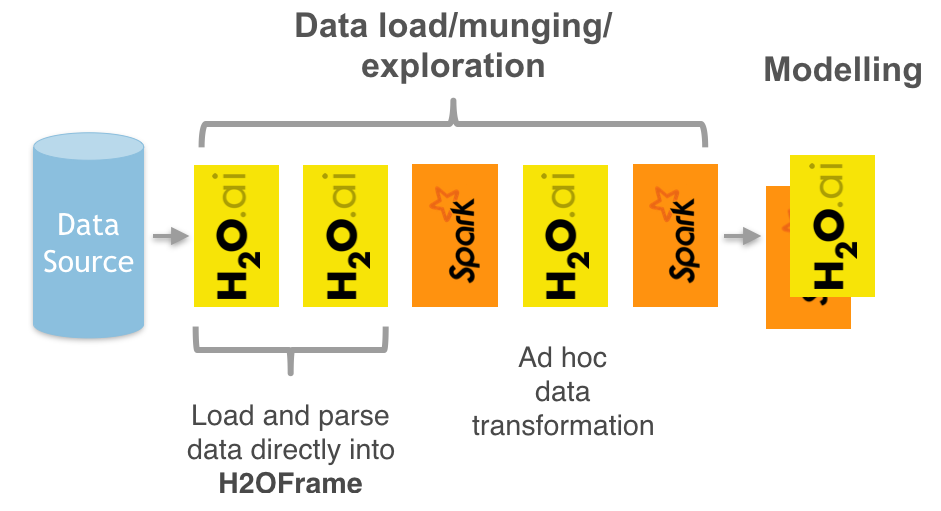
\includegraphics[scale=0.3]{../images/use-case-2.png}
        \caption{Sparkling Water introduces H2O parallel load and parse into Spark pipelines.}
        \label{fig:use-case-2}
    \end{figure}

    \subsubsection{Stream Processing}
    The last use-case depicted in Figure~\ref{fig:use-case-3} introduces two data pipelines. The first one, called
    an off-line training pipeline, is invoked regularly (e.g., every hour or every day), and utilizes both Spark and H2O API.
    The off-line pipeline provides an H2O model as output. The H2O API allows the model to be exported in a form independent
    on H2O run-time. The second pipeline processes streaming data (with help of Spark Streaming or Storm) and utilizes the
    model trained in the first pipeline to score the incoming data. Since the model is exported with no run-time dependency
    on H2O, the streaming pipeline can be lightweight and independent on H2O or Sparkling Water infrastructure.

    \begin{figure}[h!]
        \centering
        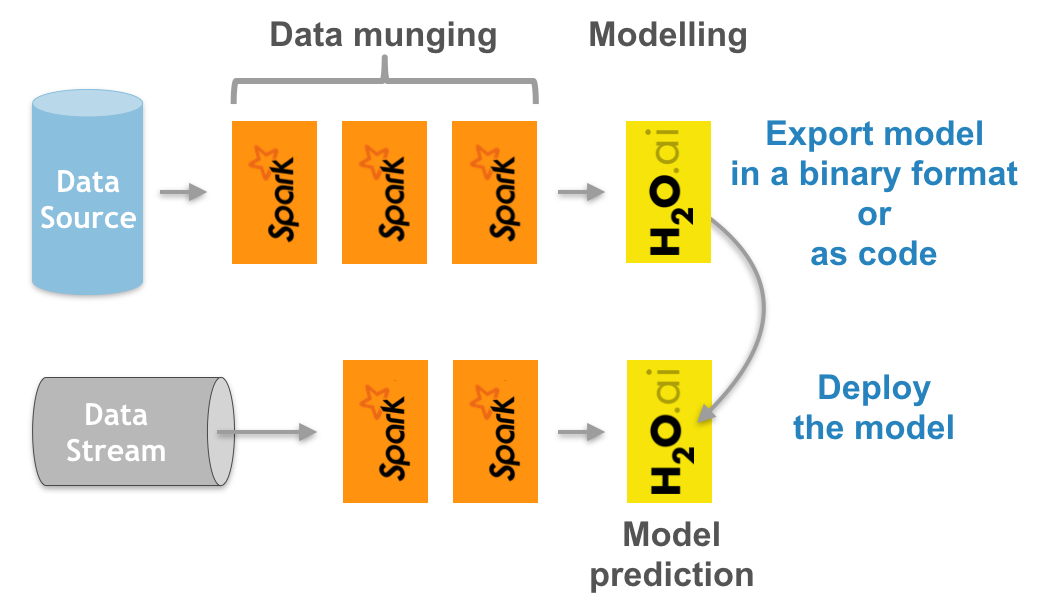
\includegraphics[scale=0.3]{../images/use-case-3.png}
        \caption{Sparkling Water used as an off-line model producer feeding models into a stream-based data pipeline.}
        \label{fig:use-case-3}
    \end{figure}

    \subsection{Features}

    Sparkling Water provides transparent integration for the H2O engine and its machine learning algorithms into
    the Spark platform, enabling:

    \begin{itemize}
        \item Use of H2O algorithms in Spark workflows
        \item Transformation between H2O and Spark data structures
        \item Use of Spark RDDs, DataFrames, and Datasets as an input for H2O algorithms
        \item Transparent execution of Sparkling Water applications on top of Spark
        \item Use H2O algorithms in Spark pipelines
        \item Productionalize H2O models in Spark environment
    \end{itemize}

    \subsection{Supported Data Sources}

    In Sparkling Water, you can either use Spark API or H2O to load data. This list describes
    all supported data sources from which Sparkling Water is able to ingest data:

    \begin{itemize}
        \item local filesystems
        \item HDFS
        \item S3
        \item HTTP/HTTPS
        \item JDBC
        \item Apache Hive
        \item DBFS (Databricks File System) when running on Databricks cluster
        \item Google Cloud Storage
    \end{itemize}

    For more details, please refer to the H2O documentation at {\url{http://docs.h2o.ai}}.

    \subsection{Supported Data Formats}

    In Sparkling Water, you can decide whether to use Spark or H2O for loading the file of the specific format.
    When using H2O API, the following formats are supported:

    \begin{itemize}
        \item CSV (delimited) files (including GZipped CSV)
        \item ORC
        \item SVMLight
        \item ARFF
        \item XLS
        \item XLSX
        \item Avro version 1.8.0 (without multi-file parsing or column type modification)
        \item Parquet
        \item Spark RDD, Data Frame or Dataset
    \end{itemize}

    For more details, please refer to the H2O documentation at {\url{http://docs.h2o.ai}}.

    \subsection{Supported Spark Execution Environments}

    Sparkling Water can run on top of Spark in the following ways:
    \begin{itemize}
        \item as a local cluster (where the master node is \texttt{local} or \texttt{local[*]})
        \item as a standalone cluster\footnote{Refer to the Spark standalone documentation
        \url{http://spark.apache.org/docs/latest/spark-standalone.html}}
        \item in a YARN environment\footnote{Refer to the Spark YARN documentation \url{http://spark.apache.org/docs/latest/running-on-yarn.html}}
    \end{itemize}

    \subsection{Sparkling Water Clients}

    Sparkling Water provides clients for R, Scala and Python languages.

    \begin{itemize}
        \item R : RSparkling
        \item Python : PySparkling
        \item Scala/Java : Sparkling Water
    \end{itemize}

    Whenever we show any code in this booklet, we will try to show variant in all three supported languages when possible.

    \subsection{Sparkling Water Requirements}

    Sparkling Water supports Spark 2.3, 2.4 (except Spark 2.4.2) and 3.0. In specific examples of this
    booklet we refer to artifacts for Spark 3.0 and use Sparkling Water 3.30.0.7, however, the Sparkling Water code is
    consistent across versions for each Spark.

    \begin{itemize}
        \item Linux/OS X/Windows
        \item Java 8 or higher
        \item Python SUBST_MIN_SUPPORTED_PYTHON+ For Python version of Sparkling Water (PySparkling)
        \item R 3.4+ for R version of Sparkling Water (RSparkling)
        \item Installed Spark and have SPARK\_HOME environmental variable pointing to its home.
    \end{itemize}
\end{document}
